\documentclass[tikz]{standalone}

\usepackage{pgfplots}


\begin{document}

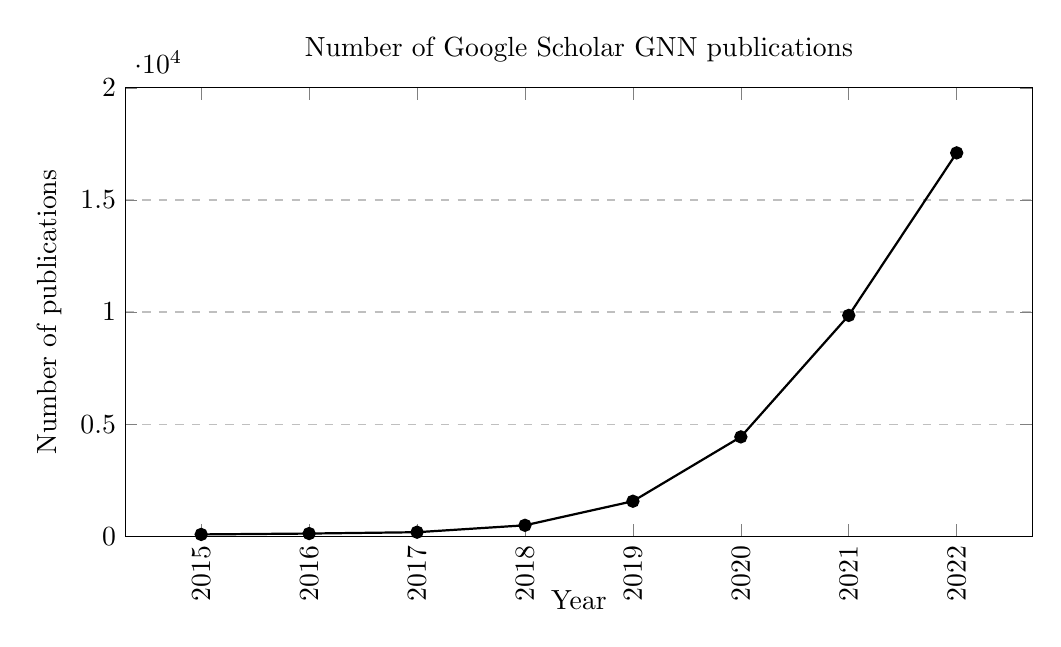
\begin{tikzpicture}
\begin{axis}[
    width=\axisdefaultheight*1.8,
    height=\axisdefaultheight,
    title={Number of Google Scholar GNN publications},
    xlabel={Year},
    x label style={at={(axis description cs:0.5,-0.1)},anchor=north},
    ylabel={Number of publications},
    ymin=0, ymax=20000,
    xticklabels={2015,2016,2017,2018,2019,2020,2021,2022},
    x tick label style={rotate=90,anchor=east},
    xtick=data,
    ytick={0,5000,10000,15000,20000},
    legend pos=north west,
    ymajorgrids=true,
    grid style=dashed,
]

\addplot[
    color=black,
    %mark=triangle*,mark options={fill=red},
    mark=*,mark options={fill=black},
    thick,
    ]
    coordinates {
    (0,79) (1, 118) (2, 178) (3, 486) (4, 1560) (5, 4430) (6, 9850) (7, 17100)
    };
    %\legend{CuSO\(_4\cdot\)5H\(_2\)O}

\end{axis}
\end{tikzpicture}

\end{document}